\begin{figure}[H]
\begin{center}
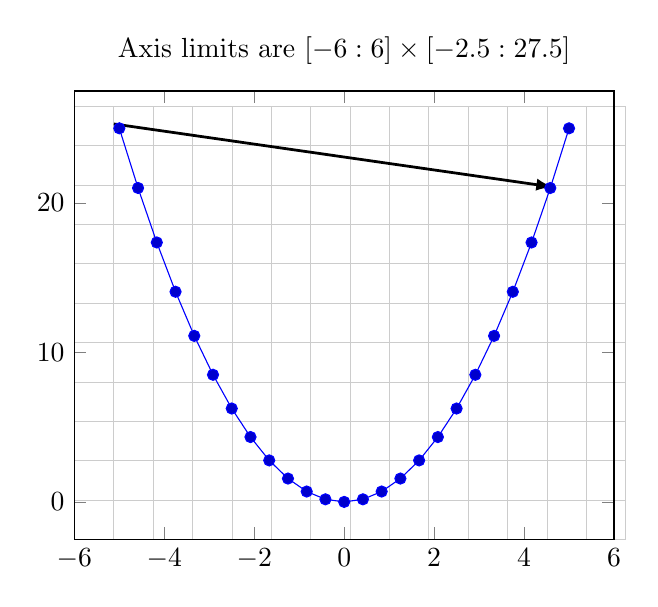
\begin{tikzpicture}
\draw[step=.5, gray!40, very thin] (0,0) grid (7,5.5);
\begin{axis}[
 % Show (automatically) computed limits:
 title={
  Axis limits are 
  $
 [\pgfmathprintnumber{\pgfkeysvalueof{/pgfplots/xmin}}
 :\pgfmathprintnumber{\pgfkeysvalueof{/pgfplots/xmax}}
 ]  \times 
 [\pgfmathprintnumber{\pgfkeysvalueof{/pgfplots/ymin}}
 :\pgfmathprintnumber{\pgfkeysvalueof{/pgfplots/ymax}}
 ]$ },
]
\addplot {x^2};
% \draw[arrows=-latex,line width=2pt] (2.8cm,-5.2cm) -- (2.8cm,.23cm);
\draw[arrows=-latex,line width=1pt] (-.07 cm,4.8cm) -- (5.5cm,4cm);
\end{axis}

    \end{tikzpicture}
  
\caption{Derivative Example }\label{fig:derivative_example}
\end{center}
\end{figure} 